\section{Challenges and Motivation}
\label{Sec:Motivation}

	In this section, we describe how \javascript code differs from traditional programming challenges and discuss challenges involved in writing and debugging \javascript code.. First we present a \javascript code example that we use as a running example throughout the paper.


	\subsection{Running Example}
	\label{Sec:Example}
			
	\figref{Example} present an example of \javascript code fragment to illustrate some of the challenges involved in providing auto-complete features for \javascript. The code fragment is based on the real world web application Wordpress.\footnote{\url{https://github.com/WordPress/WordPress/blob/master/wp-content/themes/twentytwelve/js/navigation.js}}
	
	\begin{figure}
	\medskip
	\begin{lstlisting}
	/**
 	* navigation.js
 	*
 	* Handles toggling the navigation menu for small screens.
 	*/
	( function() {
		var nav = document.getElementById( 'site-navigation' ), button, menu;
		
		button = nav.getElementsByTagName( 'h3' )[0];
		menu   = nav.getElementsByTagName( 'ul' )[0];
		if ( ! button )
			return;

		// Hide button if menu is missing or empty.
		if ( ! menu || ! menu.childNodes.length ) {
			button.style.display = 'none';
			return;
		}

		button.onclick = function() {
			if ( -1 == menu.className.indexOf( 'nav-menu' ) )
				menu.className = 'nav-menu';

			if ( -1 != button.className.indexOf( 'toggled-on' ) ) {	
				button.className = button.className.replace( ' toggled-on', '' );
				menu.className = menu.className.replace( ' toggled-on', '' );
			} else {
				button.className += ' toggled-on';
				menu.className += ' toggled-on';
			}
		};
	} )();
	\end{lstlisting}
	\caption{Example \javascript code fragment based on {\em WordPress}.}
	\label{Fig:Example}
	\end{figure}	
	
	\begin{figure}
		\centering
		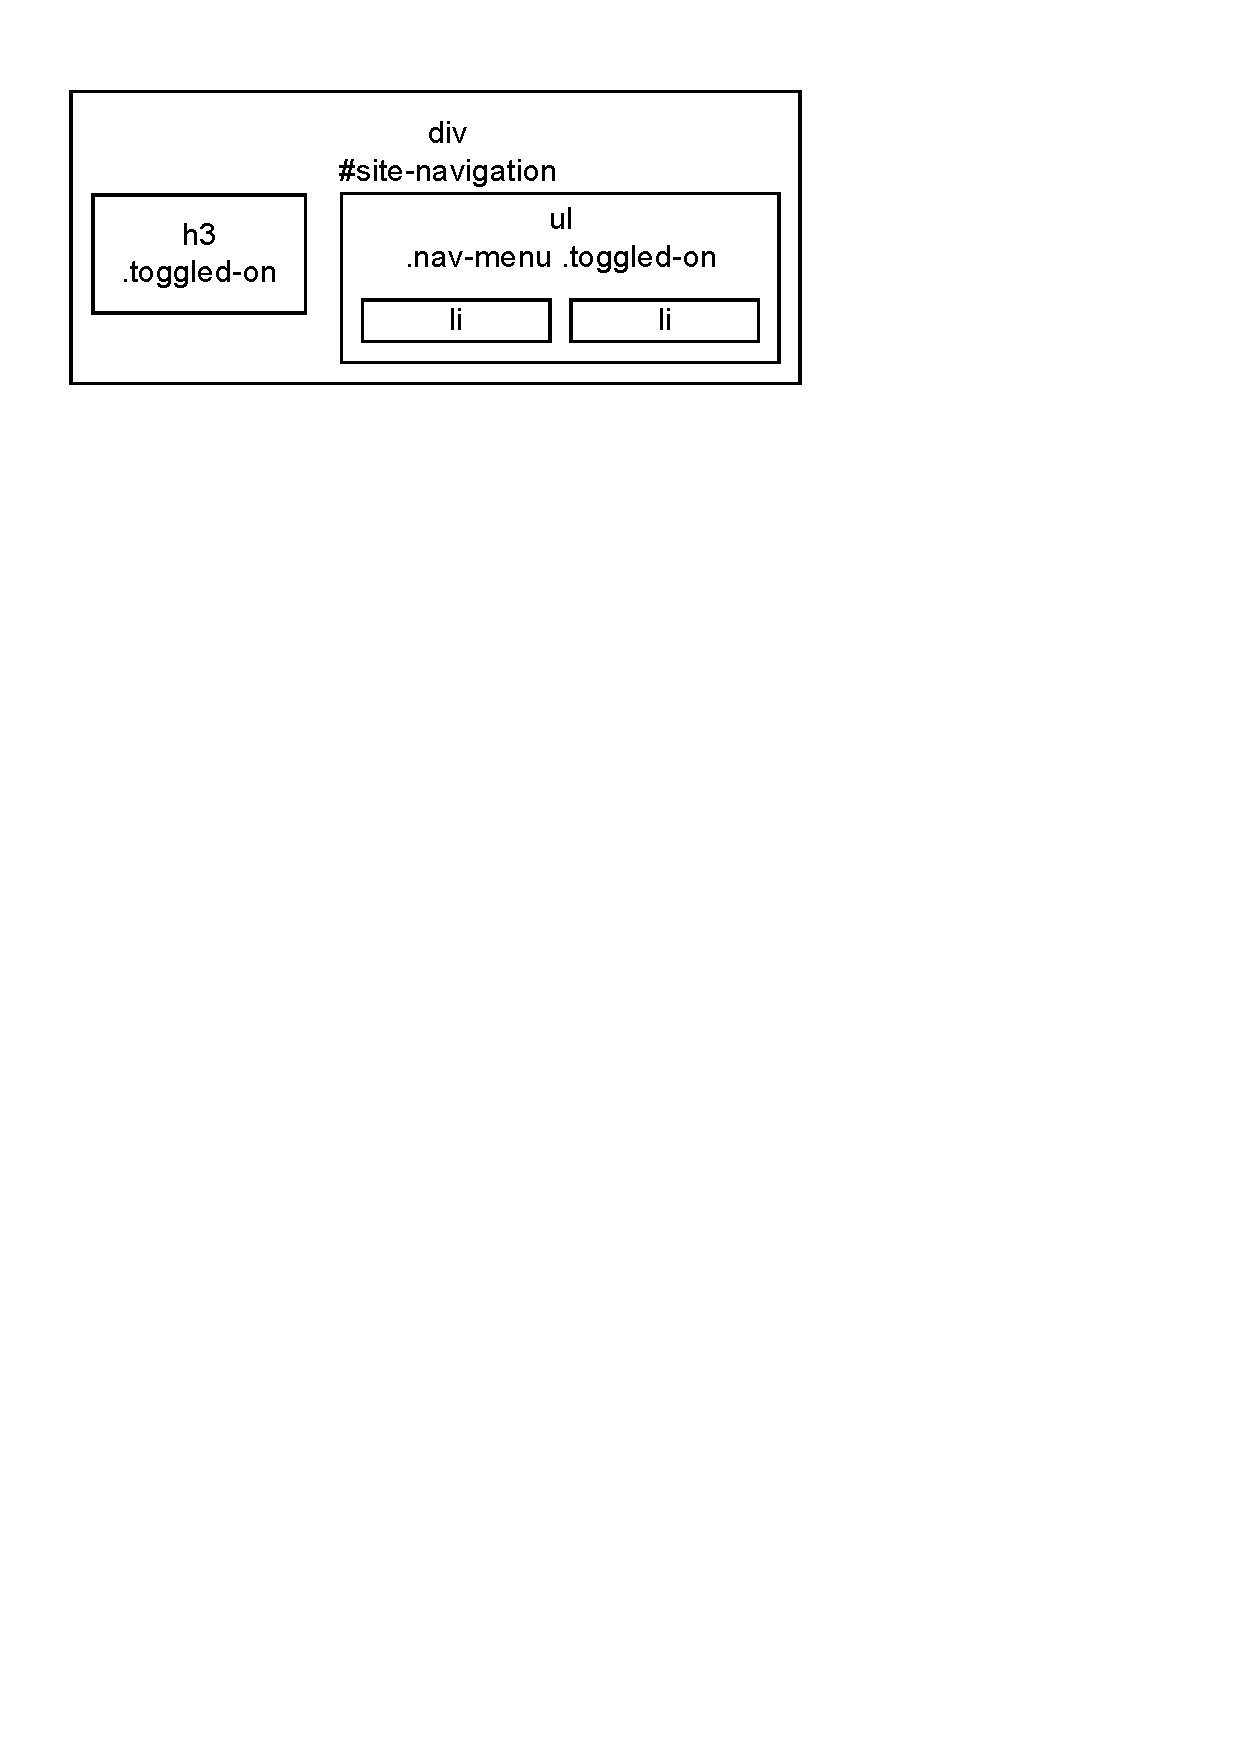
\includegraphics[width=55mm]{images/layout.pdf}
		\caption{Web page layout for the \javascript code}
		\label{Fig:Layout}
	\end{figure}

	\begin{figure}
	\medskip
	\begin{lstlisting}
	if ( ! nav )
		return;
	\end{lstlisting}
	\caption{Suggested fix}
	\label{Fig:Fix}
	\end{figure}
	
	The web application pertaining to \figref{Example} consists of a navigation menu with id \texttt{site-navigation} at the top of the web page. The navigation menu contains one \texttt{h3} element and one \texttt{ul} element that contains some \texttt{li} elements that constitute the menu items. The menu is enabled when class \texttt{toggled-on} is added to the \texttt{h3} and \texttt{ul} elements and disabled otherwise. \figref{Layout} represents the layout of the subset of web page that the \javascript code in \figref{Example} is interacting with.
	
	The \javascript code first points references to various DOM elements (Line 7-10). The code then checks for the existence of certain DOM elements and returns if these elements are not present in DOM (Line 11-18). If the elements are present, the code then attaches an \texttt{onclick} event handler to the \texttt{h3} element (Line 20) which when clicked enables / disables the navigation menu by adding and removing the class \texttt{toggled-on} (Line 24 to 30). The code also makes sure that the class \texttt{nav-menu} is attached to the \texttt{ul} element (Line 21-22). The \javascript code assumes that the DOM structure of the web page always contains an element with id \texttt{site-navigation}. Whereas the existence of \texttt{h3} and \texttt{ul} elements is not mandatory within that element.
		
	The \javascript code in \figref{Example} throws a null pointer error if navigation wrapper markup \ie element with id \texttt{site-navigation} is removed from web page header.\footnote{\url{https://core.trac.wordpress.org/ticket/22307}} This error points to the fact that the programmer was unaware of the situation when this element can be missing from the web page. To avoid this null pointer error a fix was suggested to exit the function if the navigation menu is not present on the web page. \figref{Fix} represents the suggested fix for the above mentioned error.
	
	We note that the error arises due to the lack of complete knowledge about the possible DOM states to the developer. Also, the relevant \javascript code was focussing on only specific parts of DOM (highlighted in \figref{Structure}), ignoring the rest. Therefore, DOM analysis that targets specific parts of DOM, based on the \javascript code written by the developer can be effective in detecting such errors. To eliminate such errors the developers need tools that can analyze possible DOM structures and provide suggestions to the developer. Once different parts of DOM have been analyzed in every possible DOM state, the fix for the errors similar to above error is straight forward.
	
		
	\begin{figure*}
%		\begin{mdframed}
		\centering
		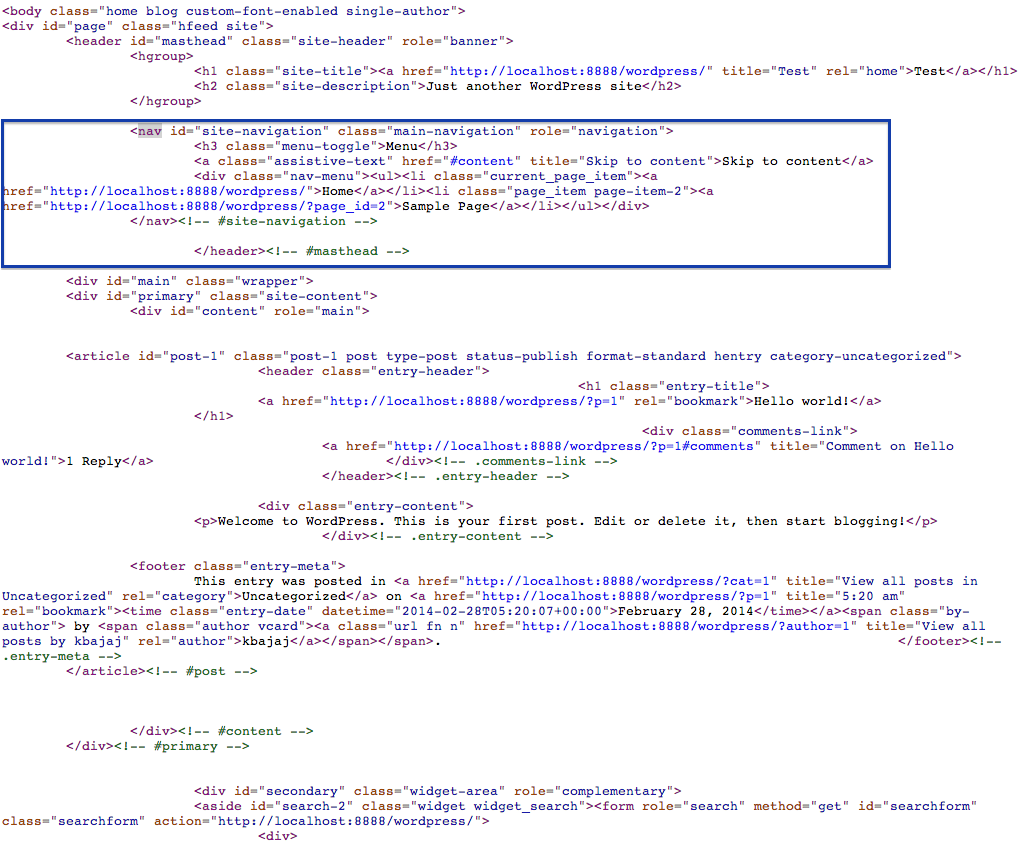
\includegraphics[width=175mm]{images/layout.png}
%		\end{mdframed}
		\caption{Overview of complete DOM Structure for the discussed example}
		\label{Fig:Structure}
	\end{figure*}
	
	\subsection{JavaScript Code Completion}
	\label{Sec:Code-completion}
	
	Although \javascript is syntactically similar to other languages such as Java, there are a number of differences that makes JavaScript different for providing code completion features.
	
	
	\headbf{Dynamically typed}
		In a dynamically typed language such as \javascript, every variable name is (unless it is null) bound only to an object. Names are bound to objects at execution time by means of assignment statements, and it is possible to bind a name to objects of different types during the execution of the program. Whereas, in case of statically typed language such as Java, every variable is bound both to a type as well as an object. Once a variable name has been bound to a type (that is, declared) it can be bound (via an assignment statement) only to objects of that type; it cannot ever be bound to an object of a different type. \figref{Typing} demonstrates the difference between strong and loose typing.

		\begin{figure}
			%\begin{mdframed}
			\centering
			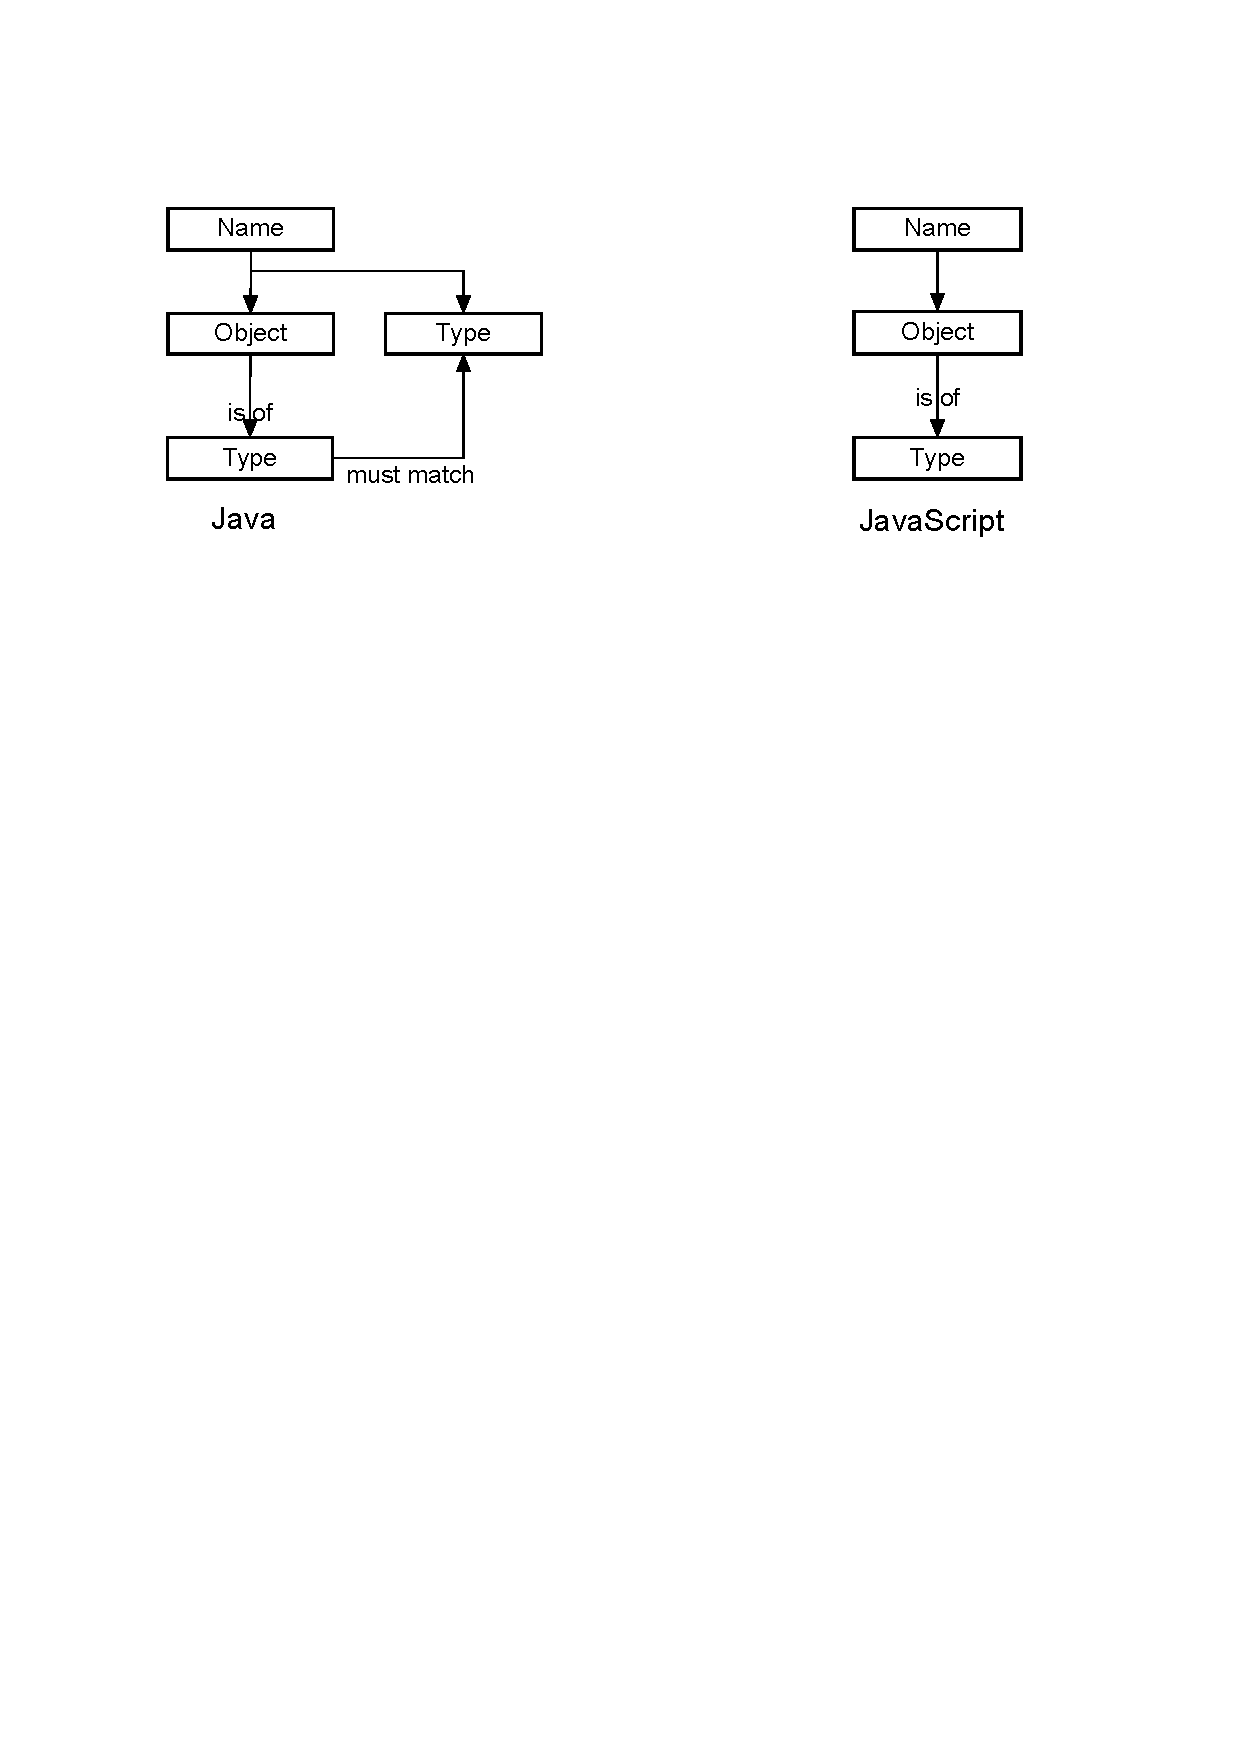
\includegraphics[width=85mm]{images/typing.pdf}
			%\end{mdframed}
			\caption{Strong typing in Java vs. Dynamic typing in \javascript}
			\label{Fig:Typing}
		\end{figure}
		
		To provide features such as code completion we need to statically analyze the code and infer variable types. For strong typed languages a single pass through the code is enough to analyze variable types as variables are declared with fixed data type. Variables once attached to a particular type remain attached throughout the code execution. Therefore, developers can provide auto-complete features just by inferring the variable types by using simple static analysis of the code. Whereas, Dynamic typed feature of \javascript makes it difficult to analyze the variable types as these types can be modified during program execution \cite{hackett2012fast, kashyap2013type}. A variable attached to \texttt{int} type at the beginning of code execution might be attached to another type by the end of the code execution. 

	
	\headbf{DOM Interactions} \javascript code frequently interacts with DOM, \ie dynamic HTML generated within the web application. In the prior work~\cite{ocariza2013empirical} we have shown the prevalence of DOM related faults in the \javascript  code. \javascript uses DOM API calls, which in return points to the DOM elements. The DOM states can be manipulated using server side code(when the page loads) as well as client side code (after the page load). Therefore, when statically analyzing the \javascript code the value of variables can either be \texttt{null} if the target element is not present in DOM or it can be value returned from the DOM, therefore changing the type of \javascript variables without any change in the \javascript code. To effectively analyze the \javascript code, the knowledge about the DOM structure is required. 
	
	\subsection{Scope of the paper}
	\label{Sec:Scope}
	
	Prior work  has shown the prevalence of \javascript errors in the production websites \cite{ocariza2011javascript}. Further analysis revealed the presence of DOM related errors within \javascript code \cite{ocariza2013empirical}. Therefore we choose to provide auto-complete suggestions for the DOM interactions within \javascript code. 
	
	\begin{table}
	{
		\scriptsize
		\begin{tabular}{ p{3.8cm} | p{3.8cm}}
  			\hline                        
  			\textbf{Function} & \textbf{Calling Objects} \\ \hline \hline
  			\texttt{getElementById()} & \texttt{document} \\ \hline
			\texttt{querySelector()} & \texttt{document, element} \\ \hline
			\texttt{getElementsByClassName()} & \texttt{document, element} \\ \hline
			\texttt{getElementsByTagName()} & \texttt{document, element} \\
  			\hline  
		\end{tabular}
	}
	\caption {DOM API for fetching DOM elements}
	\label{Table:API}		
	\end{table}

	
	In this work we focus on 4 different methods within the DOM API that can be used to point references to the DOM elements. \tabref{API} provides the list of functions used to access the DOM elements. \texttt{getElementById} function can only be called by the \texttt{document} object whereas the later 3 functions can also be called by any element within the DOM hierarchy, therefore making it possible to access any element within the DOM.
	
	
	